%
% Module 2 Chapter 3 Program Documentation
% CSC160-C00: Computer Science I (C++) (Jeffrey Hemmes)
% Author: Ashton Hellwig
% Date: 29 February 2020
%


\documentclass[a4paper, 11pt]{article}
  % Packages
  \usepackage[utf8]{inputenc}         % Encoding
  \usepackage[english]{babel}         % Internationalization
  \usepackage{times}                  % Times New Roman font
  \usepackage{soul}                   % Highlighting
  \usepackage{hyperref}               % Links (internal and external)
  \usepackage{fancyhdr}               % Headers and footers
  \usepackage[dvipsnames]{xcolor}     % Text Colors
  \usepackage{listings}               % Code Snippets
  \usepackage[section]{algorithm}     % For TOC support
  \usepackage{algpseudocode}          % Algorithmic notation environments
  \usepackage{enumitem}               % Ordered lists
  \usepackage{geometry}               % Page layout
  \usepackage{graphicx}               % Image support
  \usepackage{wrapfig}                % Sideways figures (landscape)
  \usepackage{lscape}                 % Sideways figures (landscape)
  \usepackage{rotating}               % Sideways figures (landscape)
  \usepackage{epstopdf}               % Sideways figures (landscape)
  \usepackage[toc, page]{appendix}    % Appendix
  \usepackage{setspace}               % Paragraph and line spacing
  \usepackage{bookmark}               % Required for appendix
  \usepackage{adjustbox}              % Required for appendix
  \usepackage{csquotes}               % Required for appendix
  \usepackage{amsthm}                 % Theorem environments
  \usepackage{array}                  % Arrays
  \usepackage{makecell}               % Table helpers
  \usepackage{amsmath}                % Mathematical symbols
  \usepackage[fleqn]{mathtools}       % Mathematical environments
  \usepackage{amssymb}                % Misc. symbols for logic and math
  \usepackage{relsize}                % Relative Sizing
  \usepackage{multicol}               % Multi-figure displays (grid)
  \usepackage{etoolbox,refcount}      % Required for mdframed
  \usepackage{parcolumns}             % Paragraph grids
  \usepackage{mdframed}               % Colored box environments
  \usepackage{float}                  % Floating Environments 
  \usepackage{aliascnt}               %
  % \usepackage[                        % Bibliography management
    % backend=biber,%
    % style=apa%
  % ]{biblatex}

  % Bibliography Setup
  % \addbibresource{main.bib}
  % \newcommand{\CiteSection}[2]{%
    % (\autocite{#1}, ~\S {#1})%
  % }

%   \UseRawInputEncoding

  % Tables
  \renewcommand\theadalign{bc}
  \renewcommand\theadfont{\bfseries}
  \renewcommand\theadgape{\Gape[4pt]}
  \renewcommand\cellgape{\Gape[4pt]}

  % Lists
  \newcounter{countitems}
  \newcounter{nextitemizecount}
  \newcommand{\setupcountitems}{%
    \stepcounter{nextitemizecount}%
    \setcounter{countitems}{0}%
    \preto\item{\stepcounter{countitems}}%
  }
  \makeatletter
  \newcommand{\computecountitems}{%
    \edef\@currentlabel{\number\c@countitems}%
    \label{countitems@\number\numexpr\value{nextitemizecount}-1\relax}%
  }
  \newcommand{\nextitemizecount}{%
    \getrefnumber{countitems@\number\c@nextitemizecount}%
  }
  \newcommand{\previtemizecount}{%
    \getrefnumber{countitems@\number\numexpr\value{nextitemizecount}-1\relax}%
  }
  \makeatother
  \newenvironment{AutoMultiColItemize}{%
  \ifnumcomp{\nextitemizecount}{>}{3}{\begin{multicols}{2}}{}%
  \setupcountitems\begin{itemize}}%
  {\end{itemize}%
  \unskip\computecountitems\ifnumcomp{\previtemizecount}{>}{3}{\end{multicols}}{}}



  % Colors
  \newcommand{\commentstylecolor}{\color{Gray}}
  \newcommand{\keywordstylecolor}{\color{MidnightBlue}}
  \newcommand{\stringstylecolor}{\color{ForestGreen}}
  \newcommand{\questioninput}{\color{Red}}
  \newcommand{\answertcolor}{\color{Green}}
  \newcommand{\myanswer}{\answertcolor{\hl}}

  % Symbols
  \newcommand{\answerflow}{\rotatebox[origin=c]{180}{$\Lsh$}}
  \newcommand{\toanswer}{\mathlarger{\mathlarger{\answerflow}}\quad}

  % Math
  \newcommand{\highlight}[1]{%
    \colorbox{green!50}{$\displaystyle#1$}}

  % Image Directory
  \graphicspath{ {screenshots/} }


  % Hyperlink Setup
  \hypersetup{
    colorlinks = true,
    urlcolor = blue,
    linkcolor = blue
  }


  % Algorithm Settings
  \newcommand{\pluseq}{\mathrel{{+}{=}}}
  \newcommand{\minuseq}{\mathrel{{-}{=}}}


  % Syntax-Highlighting for Code Snippets
  \lstset{
    backgroundcolor=\color{white},
    breaklines=true,%
    captionpos=b,%
    frame=tlrb,%
    tabsize=2,%
    numbers=left,%
    showstringspaces=false,%
    commentstyle=\commentstylecolor,%
    keywordstyle=\keywordstylecolor,%
    stringstyle=\stringstylecolor%
  }
  \lstset{literate=
  {á}{{\'a}}1 {é}{{\'e}}1 {í}{{\'i}}1 {ó}{{\'o}}1 {ú}{{\'u}}1
  {Á}{{\'A}}1 {É}{{\'E}}1 {Í}{{\'I}}1 {Ó}{{\'O}}1 {Ú}{{\'U}}1
  {à}{{\`a}}1 {è}{{\`e}}1 {ì}{{\`i}}1 {ò}{{\`o}}1 {ù}{{\`u}}1
  {À}{{\`A}}1 {È}{{\'E}}1 {Ì}{{\`I}}1 {Ò}{{\`O}}1 {Ù}{{\`U}}1
  {ä}{{\"a}}1 {ë}{{\"e}}1 {ï}{{\"i}}1 {ö}{{\"o}}1 {ü}{{\"u}}1
  {Ä}{{\"A}}1 {Ë}{{\"E}}1 {Ï}{{\"I}}1 {Ö}{{\"O}}1 {Ü}{{\"U}}1
  {â}{{\^a}}1 {ê}{{\^e}}1 {î}{{\^i}}1 {ô}{{\^o}}1 {û}{{\^u}}1
  {Â}{{\^A}}1 {Ê}{{\^E}}1 {Î}{{\^I}}1 {Ô}{{\^O}}1 {Û}{{\^U}}1
  {œ}{{\oe}}1 {Œ}{{\OE}}1 {æ}{{\ae}}1 {Æ}{{\AE}}1 {ß}{{\ss}}1
  {ű}{{\H{u}}}1 {Ű}{{\H{U}}}1 {ő}{{\H{o}}}1 {Ő}{{\H{O}}}1
  {ç}{{\c c}}1 {Ç}{{\c C}}1 {ø}{{\o}}1 {å}{{\r a}}1 {Å}{{\r A}}1
  {€}{{\euro}}1 {£}{{\pounds}}1 {«}{{\guillemotleft}}1
  {»}{{\guillemotright}}1 {ñ}{{\~n}}1 {Ñ}{{\~N}}1 {¿}{{?`}}1
}
  \newenvironment{alltt}{\ttfamily}{\par}
  \lstMakeShortInline[language=c++,columns=fixed]|

  % Page Configuration
  %% Style
  \pagestyle{fancy}

  %% Layout
  \geometry{%
    a4paper,%
    top=2.5cm,%
    bottom=2.5cm,%
    left=2.5cm,%
    right=2.5cm%
  }
  %%% Document
  \setlength{\headheight}{15pt}
  \setlength{\floatsep}{12pt}
  \setlength{\parindent}{2em}
  \setlength{\parskip}{0.5em}
  \renewcommand{\baselinestretch}{0.75}

  %% Title page
  \title{Chapter 3 Programming Assignment Documentation}
  \author{Ashton Hellwig}
  \date\today
  \setcounter{tocdepth}{3}

  %% Subsequent pages
  \lhead{CSC160}
  \rhead{Computer Science I (C++)}
  \lfoot{M2C3Program}
  \rfoot{A. Hellwig}


  % Document Content
\begin{document}
  % Title Page
  \maketitle
  \tableofcontents
  \listofalgorithms
  \lstlistoflistings
  \listoftables
  \newpage


  % Problem Analysis
  \section{Problem Analysis}
    The problem states:
    \begin{mdframed}[backgroundcolor=green!20]
      This assignment relates to content from Chapter 3 of the eText.

      \textbf{Instructions}\vspace{-8pt}
      \begin{enumerate}
        \item Review the general programming assignment instructions.
        \item%
          The manager of a football stadium wants you to write a program
            that calculates the total ticket sales after each game. There are
            four types of tickets -- box, sideline, premium, and general
            admission. After each game, data is stored in a file in the format
            specified in Table \ref{pa:data}.
            \begin{itemize}
              \item According to the assignment instructions, The first line
                indicates that the ticket price is \$250 and that 5750 tickets
                were sold at that price. Output the total number of tickets sold
                and the total sale amount into an output file. Format your
                output with two decimal places (You are required to generate an
                output file that has the results).
            \end{itemize}
      \end{enumerate}
    \end{mdframed}

    \subsection{Data}
      We know our output data must be output to a text document titled
        \texttt{Ch3\_Ex5Out.txt} (we chose the .txt extension to help
        reproducibility).

      \begin{table}[h!]
        \begin{tabular}{ ||l|l|| }
          \hline
          ticketPrice &numberOfTicketsSold \\
          \hline\hline
          250 &5750 \\
          100 &28000 \\
          50  &35750 \\
          25  &18750 \\
          \hline
        \end{tabular}
        \centering
        \caption{Chapter 3 Example Data}
        \label{pa:data}
      \end{table}

      \begin{enumerate}
        \item \texttt{outputData} must be formatted with two decimal places.
        \item \texttt{outputData} must be written to a file called
          ``\texttt{Ch3\_Ex5Data.txt}''.
        \item There are four tiers of tickets:
          \begin{enumerate}
            \item \texttt{box}: cost \$250 and $5750$ were sold
            \item \texttt{sideline}: cost \$100 and $28000$ were sold.
            \item \texttt{premium}: cost \$50 $35750$ were sold.
            \item \texttt{generalAdmission}: cost \$25 and $18750$ were sold.
          \end{enumerate}
      \end{enumerate}

    \subsection{Desired Output}
      \begin{lstlisting}[%
        language=bash,%
        columns=flexible,%
        caption={ashellwig\_m2c3\_programming\_assignment output (stdout)},%
        label=stdout%
    ]
Processing data...
See output file: bin/Ch3_Ex5Out.txt for the results.

Press any key to continue...
      \end{lstlisting}

      \begin{lstlisting}[%
        language=bash,%
        columns=flexible,%
        caption={%
          ashellwig\_m2c3\_programming\_assignment output (Ch3\_Ex5Out.txt)%
        },%
        label=outputdata%
    ]
Number of tickets sold = 88250
Sale amount = $6493750.00
      \end{lstlisting}


  % Algorithm
  \newpage
  \section{Algorithm}
    Below is the algorithm for the program.
    \begin{algorithm}[h]
      \caption{Chapter 3 Program Algorithm}
      \vspace{12pt}
      \begin{algorithmic}[1]
        % MAIN
        \State
        \Function{main}{}
          %% Variables
        \Comment{--Variable Declarations--}
          \State $num\gets 0$
        \EndFunction
      \end{algorithmic}
      \label{alg:c3program}
    \end{algorithm}


  % User Documentation
  \newpage
  \section{User Documentation}

    %% Usage
    \subsection{Build}
      The following are instructions with two use cases:
      \begin{itemize}
        \item With GNU Make
        \item Bundled Release
      \end{itemize}
      \subsubsection{With GNU Make}
        \begin{enumerate}
          \item Navigate to the unzipped folder containing the project,
            \textbf{with a terminal emulator or command prompt}, this will
            (most likely) mean running:
            \begin{lstlisting}[language=bash]
cd ~/Downloads/ashellwig_m2c3_programming_assignment
            \end{lstlisting}
          \item Compile the program and documentation\footnote{\textbf{Note%
            }: This requires the whole \texttt{texlive} suite as well as
            \texttt{latexmk} to be installed.} using GNU automake after
            switching to the source directory:
            \begin{lstlisting}[%
              language=bash,%
              caption={Chapter 3 Program Build Commands},%
            ]
make all # With docs
make debug # Without docs

xdg-open out/doc/user_docs.pdf # View Docs
./out/bin/ashellwig_m2c3_programming_assignment.bin # Run program

make clean-all # Removes object files, binaries, and docs
            \end{lstlisting}
          \end{enumerate}
      \subsubsection{Bundled Release}
        \begin{enumerate}
          \item Navigate to the unzipped folder containing the binary,
            \textbf{with a terminal emulator or command prompt}, this will
            (most likely) mean running:
            \begin{lstlisting}[language=bash]
cd ~/Downloads/ashellwig_m2c3_programming_assignment/bin
            \end{lstlisting}
          \item To run the program simply issue this within the command
            prompt
            \begin{lstlisting}[language=bash]
./build/ashellwig_m2c3_programming_assignment
            \end{lstlisting}
        \end{enumerate}
        Of course if preferred, you may also navigate to the build folder in
          file explorer and double click the executable
          (\texttt{./ashellwig\_m2c3\_programming\_assignment}).


  % Appendix
  % \newpage
  % \appendix

  % Images
  % \section{Images}
    % \begin{sidewaysfigure}[ht]
      % 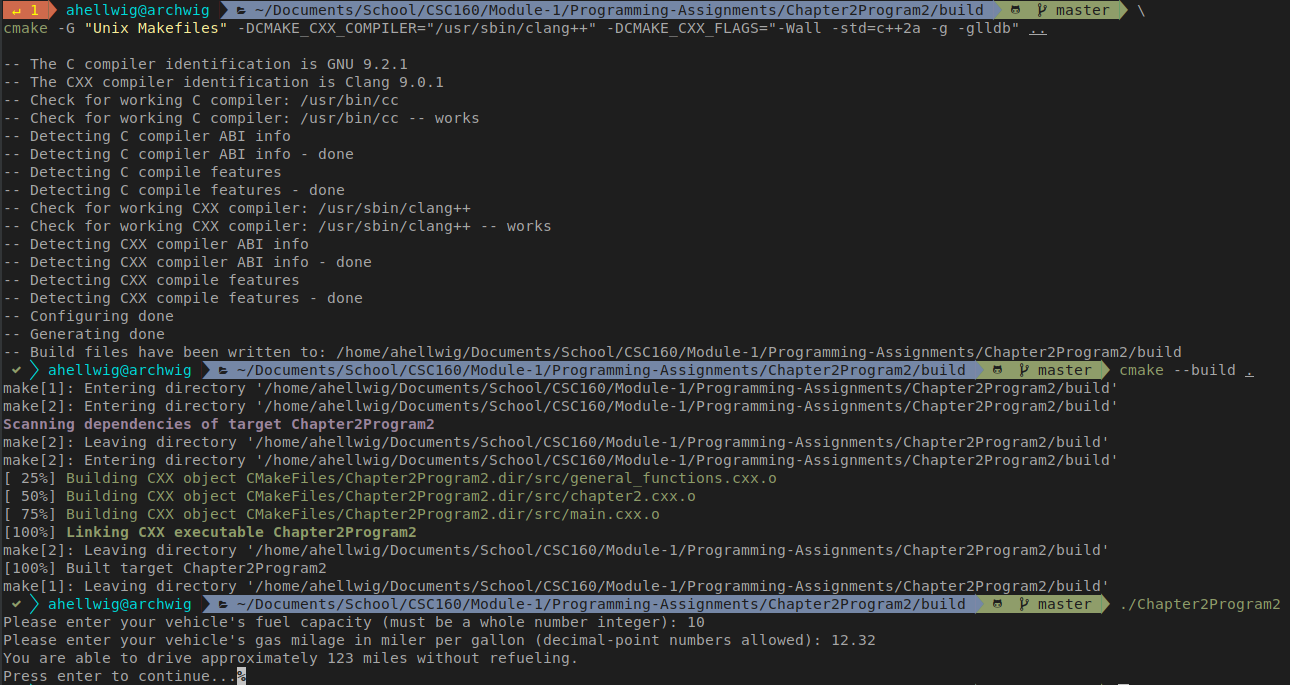
\includegraphics[%
      %   width={1000px}%
      % ]{compandrun.png}
    % \end{sidewaysfigure}
\end{document}
